\subsection{Reactome pathway audit with controls fixed in advance: two gates failed, verdicts inconclusive}
We repeated the pathway question with Reactome v97 (AnalysisService projection; \texttt{scripts/reactome\_enrichment.py}; \texttt{results/reactome\_enrichment.json}; hermetic tests), this time with the site-count and expression-matched controls pre-registered. Per miRNA we count pathways at entities FDR $<0.05$ for CNN top-200, site-count top-200, three expression-matched and three uniform random sets.
Two of three gates failed as written. G1 required a pathway named ``Cell Cycle'' among the top three for a 20-gene cell-cycle control; the control returned 205 significant pathways, but the top three are tied at the same FDR and none has that name (a post-hoc look finds 7 such pathways lower in the list). G3 required fewer than 10\% unmapped genes; the median is 39.8\%, because Reactome curates only part of the genome. Both are design errors on our side, and we do not rewrite the gates. G2 passed (median uniform-set count 0).
Under failed gates we report the numbers but call the audit inconclusive: CNN versus uniform random 3/6 ($p=0.910$), versus site count 2/2 ($p=0.688$), versus expression-matched 4/6 ($p=0.828$). Most sets in every arm have zero significant pathways, with a few large random-set outliers (Figure~\ref{fig:reactome}). None of this points toward pathway coherence, which agrees with the g:Profiler result.
\begin{figure}[h]\centering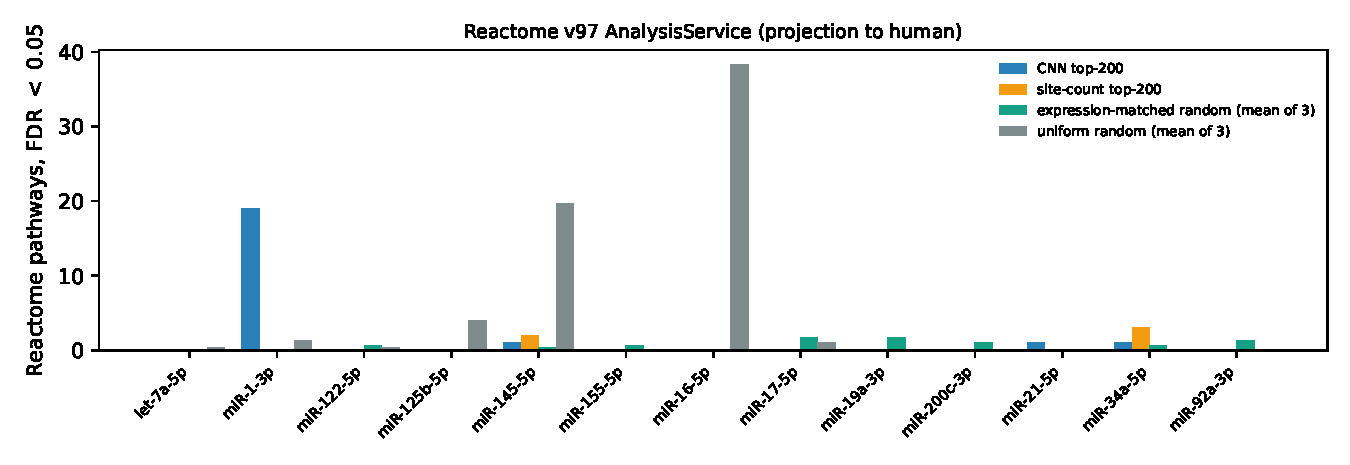
\includegraphics[width=0.95\linewidth]{figs/fig_reactome.pdf}
\caption{Significant Reactome pathways per miRNA for four arms of 200 genes. Gates G1 and G3 failed, so these counts are descriptive.}\label{fig:reactome}\end{figure}
